\chapter{Arhitektura i dizajn sustava}
		
		Arhitektura sustava može se podijelit na tri glavna podsustava: web preglednik, web poslužitelj i baza podataka.
	\begin{itemize}
		\item 	\textbf{Web preglednik} – program koji služi za pristupanje web stranicama. Putem web preglednika korisnik komunicira sa poslužiteljem koristeći princip zahtjev-odgovor ili šalje podatke (najčešće u obliku obrazaca). Daljnja zadaća web preglednika je osigurati da se traženi podaci ispravno prikazuju ili da se ispravno prosljeđuju i spremaju na poslužitelj.
		\item 	\textbf{Web poslužitelj} – glavni je dio web aplikacije. To je most koji povezuje korisnika i bazu podataka koji se temelji na protokolu HTTP. Na zahtjeve korisnika dohvaća tražene podatke (resurse) ili obrađuje i sprema poslane podatke od korisnika.
		\item 	\textbf{Baza podataka} – srce je sustava. U njoj su pospremljeni svi podaci. Skoro ne postoji sustav u kojem nema komunikacije između aplikacije i baze.	
	\end{itemize}
		Aplikacije je izgrađena na modelu MVC (Model – View - Controller) softverske arhitekture uz male modifikacije. Controller dio strukture je ostvaren tako što je integriran unutar same baze. Shodno tome aplikaciju onda dijelimo na tri komponente:
	\begin{itemize}
		\item	\textbf{Model} – glavna komponenta sustava. Čuva razrede čiji se objekti obrađuju.
		\item	\textbf{View} – komponenta zaslužna za reprezentaciju podataka.
		\item	\textbf{Controller} – komponenta koja odrađuje svu logiku i komunikaciju između sučelja i baze.
	\end{itemize}
	
		\smallskip
		Programski jezik koji smo odabrali za izradu backend-a naše aplikacije je ????, zajedno sa REST API-em za komunikaciju sa bazom. Za izradu fronend-a korišteni su ??????. Od vanjskih servisa smo integrirali podršku za korištenje Google Maps-a. Razvojno okruženje koje smo koristili je bilo Visual Studio Code.
		

		

				
		\section{Baza podataka}
			
			%\textbf{\textit{dio 1. revizije}}\\
			
		%\textit{Potrebno je opisati koju vrstu i implementaciju baze podataka ste odabrali, glavne komponente od kojih se sastoji i slično.}
			U ovom projektu koristit ćemo relacijsku bazu podataka, čije su osnovne jedinke entiteti, definirani imenom i skupom atributa. Osnovna zadaća baze podataka je pohrana podataka te brza i efikasna obrada tih podataka u ovisnosti i korisničkim zahtjevima. U bazi podataka su pohranjeni podaci o korisnicima, njihovim ulogama, preferencijama, kao i o smještaju te dostupnosti smještaja. Dodatno uz navedeno, zbog zahtjeva organizacije prijevoza, baza također sprema informacije o vrstama vozila i dostupnosti tih vozila kao i o vremenu i mjestu boravka korisnika zdravstvenog turizma. Tako su i definirani sljedeći entiteti:
			\begin{itemize}
				\item Clinic
				\item Town
				\item AdminUser
				\item Credentials
				\item UserRole
				\item Patient
				\item Treatment
				\item PatientPreferences
				\item Accomodation
				\item AccomodationType
				\item Equipped
				\item AccomodationOccupied
				\item Transporter
				\item Vehicle
				\item VehicleType
				\item VehicleOccupied
				\item VehicleAvaliability
			\end{itemize}
		
			\subsection{Opis tablica}
			
				%clinic
				\textbf{Clinic} Ovaj entitet sadrži podatke o klinikama u odabranoj zemlji. Atributi su: ClinicID (primary key), clinicName, latitude, longitude, clinicAddress, TownID (foreign key). Ovaj je entitet u vezi Many-to-One sa entitetom Town preko atributa TownID, u Many-to-Many vazi sa entitetom Accomodation preko atributa AccomodationID i ClinicID, u Many-to-Many vezi sa entitetom Transporter preko atributa TransporterID i ClinicID , u One-to-Many vezi sa entitetom Patient preko atributa PatientID i ClinicID te u Many-to-Many vezi sa entitetom Treatment preko atributa TreatmentID.
				
				\begin{longtblr}[
					label=none,
					entry=none
					]{
						width = \textwidth,
						colspec={|X[8,l]|X[6, l]|X[20, l]|}, 
						rowhead = 1,
					} %definicija širine tablice, širine stupaca, poravnanje i broja redaka naslova tablice
					\hline \SetCell[c=3]{c}{\textbf{Clinic}}	 \\ \hline[3pt]
					\SetCell{LightGreen}ClinicID & BIGSERIAL & Jedinstveni brojčani identifikator klinike,automatski generiran \\ \hline
					clinicName & VARCHAR & Ime klinike	\\ \hline  
					Latitude & DECIMAL	& Geografska širina	\\ \hline 
					Longitude & DECIMAL & Geografska dužina \\ \hline
					clinicAddress & VARCHAR & Adresa klinike  \\ \hline
					\SetCell{LightBlue}TownID & INT & Grad u kojem se klinika nalazi \\ \hline
				\end{longtblr}
				
				%Town
				\textbf{Town} Ovaj entitet sadrži podatke o gradovima u kojima se nalaze klinike u koje dolaze pacijenti na liječenje. Atributi su: TownID (primary key) i townName. Ovaj entitet je u vezi One-to-Many sa entitetom Clinic preko atributa TownID i u vezi One-to-Many sa entitetom Accomodation preko atributa TownID i u Many-to-Many vezi sa entitetom Transporter preko atributa TownID.
				
				\begin{longtblr}[
					label=none,
					entry=none
					]{
						width = \textwidth,
						colspec={|X[8,l]|X[6, l]|X[20, l]|}, 
						rowhead = 1,
					} %definicija širine tablice, širine stupaca, poravnanje i broja redaka naslova tablice
					\hline \SetCell[c=3]{c}{\textbf{Town}}	 \\ \hline[3pt]
					\SetCell{LightGreen}TownID & BIGSERIAL & Jedinstveni brojčani identifikator grada, automatski generiran \\ \hline
					townName & VARCHAR & Ime grada	\\ \hline 
				\end{longtblr}
				
				\newpage
				
				%AdminUser
				\textbf{AdminUser} Ovaj entitet sadrži podatke o korisnicima aplikacije; svi administratori i oni koji mogu dodavati ili ažurirati ili brisati podatke iz baze. Atributi su: UserID (primary key), PIN(personal identification number), firstname, lastname, phone, email. Ovaj je entitet u vezi Many-to-Many sa entitetom UserRole preko atributa RoleID te u vezi One-to-One sa entitetom Credentials preko atributa UserID.
				
				\begin{longtblr}[
					label=none,
					entry=none
					]{
						width = \textwidth,
						colspec={|X[8,l]|X[6, l]|X[20, l]|}, 
						rowhead = 1,
					} %definicija širine tablice, širine stupaca, poravnanje i broja redaka naslova tablice
					\hline \SetCell[c=3]{c}{\textbf{AdminUser}}	 \\ \hline[3pt]
					\SetCell{LightGreen}UserID & BIGSERIAL & Jedinstveni brojčani identifikator korisnika, automatski generiran \\ \hline
					PIN & INT & Identifikacijski broj korisnika	\\ \hline 
					firstname & VARCHAR & Ime korisnika  \\ \hline 
					lastname & VARCHAR & Prezime korisnika	\\ \hline 
					phone & VARCHAR & Broj mobitela korisnika \\ \hline
					email & VARCHAR & Elektronička pošta korisnika \\ \hline
				\end{longtblr}
				
				%Credentials
				\textbf{Credentials} Ovaj entitet sadrži podatke o korisničkim računima administratora. Atributi su: UserID (foreign key), username i pass. Ovaj je entitet u One-to-One vezi sa entitetom AdminUser preko atributa UserID.
				
				\begin{longtblr}[
					label=none,
					entry=none
					]{
						width = \textwidth,
						colspec={|X[8,l]|X[6, l]|X[20, l]|}, 
						rowhead = 1,
					} %definicija širine tablice, širine stupaca, poravnanje i broja redaka naslova tablice
					\hline \SetCell[c=3]{c}{\textbf{Credentials}}	 \\ \hline[3pt]
					\SetCell{LightBlue}UserID & BIGSERIAL & ID korisnika kojem pripadaju korisničko ime i lozinka \\ \hline
					username & VARCHAR & Jedinstveno korisničko ime \\ \hline
					pass & BINARY & Lozinka korisnika za prijavu u aplikaciju	\\ \hline 
				\end{longtblr}

				\newpage

				%UserRole
				\textbf{UserRole} Ovaj entitet sadrži podatke o ulogama koje postoje u sustavu. Atributi su: RoleID i roleName. Ovaj je entite u Many-to-One vezi sa entitetom UserAdmin preko atributa UserID.
				
				\begin{longtblr}[
					label=none,
					entry=none
					]{
						width = \textwidth,
						colspec={|X[8,l]|X[6, l]|X[20, l]|}, 
						rowhead = 1,
					} %definicija širine tablice, širine stupaca, poravnanje i broja redaka naslova tablice
					\hline \SetCell[c=3]{c}{\textbf{UserRole}}	 \\ \hline[3pt]
					\SetCell{LightGreen}RoleID & SMALLINT & Jedinstveni indentifikator uloge, automatski generiran \\ \hline
					roleName & VARCHAR & ime uloge \\ \hline 
				\end{longtblr}
				
				%Patient
				\textbf{Patient} Ovaj entitet sadrži podatke o korisnicima zdravstvenog turizma. Atributi su: PatientID (primary key), PIN (personal identification number), firstname, lastname, phone, email, residenceAddress. Ovaj je entitet u vezi One-to-One sa entitetom Accomodation preko atributa AccomodationID, u vezi One-to-Many vezi sa entitetom Treatment preko atributa TreatmentID te u One-to-Many vezi sa entitetom Clinic preko atributa ClinicID i PatietnID.
				
				\begin{longtblr}[
					label=none,
					entry=none
					]{
						width = \textwidth,
						colspec={|X[8,l]|X[6, l]|X[20, l]|}, 
						rowhead = 1,
					} %definicija širine tablice, širine stupaca, poravnanje i broja redaka naslova tablice
					\hline \SetCell[c=3]{c}{\textbf{Patient}}	 \\ \hline[3pt]
					\SetCell{LightGreen}PatientID & BIGSERIAL & Jedinstveni brojčani identifikator pacijenta, automatski generiran \\ \hline
					PIN & INT & Identifikacijski broj pacijenta	\\ \hline 
					firstname & VARCHAR & Ime pacijenta  \\ \hline 
					lastname & VARCHAR & Prezime pacijenta	\\ \hline 
					phone & VARCHAR & Broj mobitela pacijenta \\ \hline
					email & VARCHAR & Elektronička pošta pacijenta \\ \hline
					residenceAddress & VARCHAR & Mjesto prebivališta pacijenta \\ \hline
				\end{longtblr}
				
				\newpage
				
				%Treatment
				\textbf{Treatment} Ovaj entitet sadrži podatke o tretmanima. Atributi su: TreatmentID (primary key) i description. Ovaj je entite u Many-to-One vezi sa entitetom Patient preko atributa TreatmentID i PatientID te u One-to-Many vezi sa entitetom Clinic preko atributa TreatmentID i ClinicID.
				
				\begin{longtblr}[
					label=none,
					entry=none
					]{
						width = \textwidth,
						colspec={|X[8,l]|X[6, l]|X[20, l]|}, 
						rowhead = 1,
					} %definicija širine tablice, širine stupaca, poravnanje i broja redaka naslova tablice
					\hline \SetCell[c=3]{c}{\textbf{Treatment}}	 \\ \hline[3pt]
					\SetCell{LightGreen}TreatmentID & BIGSERIAL & Jedinstveni indentifikator tretmana, automatski generiran \\ \hline
					description & text & opsi tretmana \\ \hline 
				\end{longtblr}
				
					%PatientPreferences
				\textbf{PatientPreferences} Ovaj entitet sadrži podatke o preferencijama pacijenta vezanih za smještaj. Atributi su: PatientID (foreign key), TypeID (foreign key), EquippedID (foreign key). Ovaj je entite u Many-to-One vezi sa entitetom Patient preko atributa PatientID, u One-to-One vezi sa entitetom AccomodationType preko atributa AccomodationID te u One-to-One vezi sa entitetom Equipped preko atributa EquippedID.
				
				\begin{longtblr}[
					label=none,
					entry=none
					]{
						width = \textwidth,
						colspec={|X[8,l]|X[6, l]|X[20, l]|}, 
						rowhead = 1,
					} %definicija širine tablice, širine stupaca, poravnanje i broja redaka naslova tablice
					\hline \SetCell[c=3]{c}{\textbf{PatientPreferences}}	 \\ \hline[3pt]
					\SetCell{LightBlue}PatientID & BIGSERIAL & Jedinstveni indentifikator pacijenta, automatski generiran \\ \hline
					\SetCell{LightBlue}TypeID & SMALLINT & Jedinstveni indentifikator vrste smještaja, automatski generiran \\ \hline
					\SetCell{LightBlue}EquippedID & SMALLINT & Jedinstveni indentifikator opremljenosti smještaja, automatski generiran \\ \hline
				\end{longtblr}
				
				%Accomodation
				\textbf{Accomodation} Ovaj entitet sadrži podatke o smještaju, vrsti smještaja, njegovoj opremljenosti te adresi na kojoj se nalazi kao i koordinatama. Atributi su: AccomodationID (primary key), TypeID (foreign key), EquippedID (foreing key), latitude, longitude, address, TownID (foreign key), active. Ovaj je entitet u vezi Many-to-One sa entitetom Town preko atributa TownID, nadalje u vezi Many-to-One sa entitetom AccomodationType preko atributa TypeID, u vezi Many-to-One sa entitetom Equipped preko atributa EquippedID, u vezi One-to-One sa entitetom Patient preko atributa AccomodationID i PatientID.
				
				\begin{longtblr}[
					label=none,
					entry=none
					]{
						width = \textwidth,
						colspec={|X[8,l]|X[6, l]|X[20, l]|}, 
						rowhead = 1,
					} %definicija širine tablice, širine stupaca, poravnanje i broja redaka naslova tablice
					\hline \SetCell[c=3]{c}{\textbf{Accomodation}}	 \\ \hline[3pt]
					\SetCell{LightGreen}AccomodationID & BIGSERIAL & Jedinstveni brojčani identifikator smještaja, automatski generiran \\ \hline
					\SetCell{LightBlue} TypeID & INT & ID vrste smještaja \\ \hline
					\SetCell{LightBlue} EquippedID & INT & ID opremljenosti smještaja \\ \hline
					latitude & DECIMAL & Geografska širina  \\ \hline 
					longitude & DECIMAL & Geografska dužina	\\ \hline 
					address & VARCHAR & Adresa smještaja	\\ \hline
					\SetCell{LightBlue} TownID & INT & ID grada u kojem se smještaj nalazi \\ \hline
					active & BIT & Je li smještaj upotrebljiv \\ \hline
				\end{longtblr}
				
				%AccomodationType
				\textbf{AccomodationType} Ovaj entitet sadrži podatke o tipu smještaja (stan u zgradi, stan u kući, iznajmljeno, u vlasništvu klinike). Atributi su: TypeID (primary key), description. Ovaj je entitet u One-to-Many vezi s entitetom Accomodation preko atributa TypeID.
				
				\begin{longtblr}[
					label=none,
					entry=none
					]{
						width = \textwidth,
						colspec={|X[8,l]|X[6, l]|X[20, l]|}, 
						rowhead = 1,
					} %definicija širine tablice, širine stupaca, poravnanje i broja redaka naslova tablice
					\hline \SetCell[c=3]{c}{\textbf{AccomodationType}}	 \\ \hline[3pt]
					\SetCell{LightGreen}TypeID & SMALLINT & Jedinstveni identifikator vrste smještaja, automatski generiran \\ \hline
					description & TEXT & Opis vrste smještaja (stan u kući, stan u zgradi, soba u hotelu ili motelu)	\\ \hline 
				\end{longtblr}
				
				%Equipped
				\textbf{Equipped} Ovaj entitet sadrži podatke o vrsti opremljenosti smještaja (potpuno opremljen, djelomično opremljen). Atributi su: EquippedID (primary key), equipment. Ovaj je entitet u One-to-Many vezi sa entitetom Accomodation preko atributa EquippedID.
				
				\begin{longtblr}[
					label=none,
					entry=none
					]{
						width = \textwidth,
						colspec={|X[8,l]|X[6, l]|X[20, l]|}, 
						rowhead = 1,
					} %definicija širine tablice, širine stupaca, poravnanje i broja redaka naslova tablice
					\hline \SetCell[c=3]{c}{\textbf{Equipped}}	 \\ \hline[3pt]
					\SetCell{LightGreen}EquippedID & SMALLINT & Jedinstveni identifikator opremljenosti smještaja, automatski generiran \\ \hline
					equipment & TEXT & Opis opremljenosti smještaja (potpuno opremljen, djelomično opremljen)	\\ \hline 
				\end{longtblr}
				
				%AccomodationOccupied
				\textbf{AccomodationOccupied} Ovaj entitet sadrži podatke o zauzetosti smještaja kojima raspolaže pojedina klinika. Atributi su: PatientID (foreign key), AccomodationID (foreign key), dateTo, dateFrom. Ovaj je entitet u One-to-One vezi sa entitetom Accomodation preko atributa AccomodationID te u One-to-One vezi sa entiteom Patient preko atributa PatientID.
				
				\begin{longtblr}[
					label=none,
					entry=none
					]{
						width = \textwidth,
						colspec={|X[8,l]|X[6, l]|X[20, l]|}, 
						rowhead = 1,
					} %definicija širine tablice, širine stupaca, poravnanje i broja redaka naslova tablice
					\hline \SetCell[c=3]{c}{\textbf{AccomodationOccupied}}	 \\ \hline[3pt]
					\SetCell{LightBlue}PatientID & BIGSERIAL & Jedinstveni identifikator pacijenta \\ \hline
					\SetCell{LightBlue}AccomodationID & BIGSERIAL & Jedinstveni identifikator smještaja \\ \hline
					dateFrom & DATE & Datum od kojeg je smještaj dostupan \\ \hline
					dateTo & DATE & Datum do kojeg je smještaj dostupan \\ \hline 
				\end{longtblr}
				
				%Transporter
				\textbf{Transporter} Ovaj entitet sadrži podatke o prijevoznicima s kojima klinika ima ugovore za prijevoz pacijenata. Atributi su: TransporterID (primary key), organisationName, phone, address, TownID (foreign key), active. Ovaj je entitet u Many-to-Many vezi sa entitetom Town preko atributa TownID, u Many-to-Many vezi sa entitetom Clinic preko atributa ClincID te u One-to-Many vezi sa entitetom Vehicle preko atributa TransporterID.
				
				\begin{longtblr}[
					label=none,
					entry=none
					]{
						width = \textwidth,
						colspec={|X[8,l]|X[6, l]|X[20, l]|}, 
						rowhead = 1,
					} %definicija širine tablice, širine stupaca, poravnanje i broja redaka naslova tablice
					\hline \SetCell[c=3]{c}{\textbf{Transporter}}	 \\ \hline[3pt]
					\SetCell{LightGreen}TransporterID & BIGSERIAL & Jedinstveni identifikator prijevoznika, automatski generiran \\ \hline
					organisationName & VARCHAR & Ime prijevoznika \\ \hline
					phone & VARCHAR & Broj mobitela prijevoznika \\ \hline
					address & VARCHAR & Adresa baze prijevoznika \\ \hline
					\SetCell{LightBlue} TownID & INT & ID grada u kojem se smještaj nalazi \\ \hline
					active & BIT & Je li prijevoznik radi \\ \hline
				\end{longtblr}
				
				%Vehicle
				\textbf{Vehicle} Ovaj entitet sadrži podatke o vozilima kojima transporter raspolaže. Atributi su: VehicleID (primary key), capacity TypeID (foreign key), TransporterID (foreign key) te active. Ovaj je entitet u Many-to-One vezi sa entitetom Transporter preko atributa TransporterID, u Many-to-Many vezi sa entitetom VehicleOccupied preko atributa VehicleID, u One-to-One vezi sa entitetom VehicleType preko atributa VehicleID te u One-to-Manz vezi sa entitetom VehicleAvaliability preko atributa VehicleID.
				
				\begin{longtblr}[
					label=none,
					entry=none
					]{
						width = \textwidth,
						colspec={|X[8,l]|X[6, l]|X[20, l]|}, 
						rowhead = 1,
					} %definicija širine tablice, širine stupaca, poravnanje i broja redaka naslova tablice
					\hline \SetCell[c=3]{c}{\textbf{Vehicle}}	 \\ \hline[3pt]
					\SetCell{LightGreen}VehicleID & BIGSERIAL & Jedinstveni identifikator vozila, automatski generiran \\ \hline
					capacity & SMALLINT & Kapacitet vozila (2 osobe, 4 osobe, 5 osoba….) \\ \hline
					\SetCell{LightBlue}TypeID & SAMLLINT & Vresta vozila \\ \hline
					\SetCell{LightBlue}TransporterID & INT & Jedinstveni identifikator prijevoznika kojem vozilo pripada \\ \hline
					active & BIT & Je li vozilo u funkciji \\ \hline
				\end{longtblr}
				
				%VehicleType
				\textbf{VehicleType} Ovaj entitet sadrži podatke o vrsti vozila. Atributi su: TypeID(primary key), description. Ovaj je entitet u One-to-One vezi sa entitetom Vehicele preko atributa VehicleID.
				
				\begin{longtblr}[
					label=none,
					entry=none
					]{
						width = \textwidth,
						colspec={|X[8,l]|X[6, l]|X[20, l]|}, 
						rowhead = 1,
					} %definicija širine tablice, širine stupaca, poravnanje i broja redaka naslova tablice
					\hline \SetCell[c=3]{c}{\textbf{VehicleType}}	 \\ \hline[3pt]
					\SetCell{LightGreen}TypeID & SMALLINT & Jedinstveni identifikator vrste vozila, automatski generiran \\ \hline
					description & TEXT & Opis vrste vozila (auto, kombi, min-bus...) \\ \hline
				\end{longtblr}
				
				\newpage
				
				%VehicleOccupied
				\textbf{VehicleOccupied} Ovaj entitet sadrži podatke o vremenima kada je koje vozilo zauzeto, tj. kada prevozi pacijente od smještaja do klinike te natrag. Atributi su: VehicleID (foreign key), PatientID (foreign key), timeStart, timeEnd. Ovaj je entitet u One-to-Many vezi sa entitetom Vehicle preko atributa VehicleID te u One-to-One vezi sa entitetom Patient preko atributa PatientID.
				
				\begin{longtblr}[
					label=none,
					entry=none
					]{
						width = \textwidth,
						colspec={|X[8,l]|X[6, l]|X[20, l]|}, 
						rowhead = 1,
					} %definicija širine tablice, širine stupaca, poravnanje i broja redaka naslova tablice
					\hline \SetCell[c=3]{c}{\textbf{VehicleOccupied}}	 \\ \hline[3pt]
					\SetCell{LightBlue}VehicleID & INT & Jedinstveni identifikator vozila koje je zauzeto \\ \hline
					\SetCell{LightBlue}PatientID & INT & Jedinstveni identifikator pacijenta kojem je vozilo dodijeljeno \\ \hline
					timeStart & TIME & Vrijem od kada je vozilo zauzeto \\ \hline
					timeEnd & TIME & Vrijeme do kada je vozilo zauzeto \\ \hline
				\end{longtblr}
				
				%VehicleAvaliability
				\textbf{VehicleAvaliability} Ovaj entitet sadrži podatke o vremenima kada je koje vozilo dostupno, tj. radno vrijeme radnih dana. Atributi su: VehicelID (foreign key), DOW (day of the week), tiemStart, timeEnd. Ovaj je entitet u Many-to-Many vezi sa entitetom Vehicle preko atributa VehicleID.
				
				\begin{longtblr}[
					label=none,
					entry=none
					]{
						width = \textwidth,
						colspec={|X[8,l]|X[6, l]|X[20, l]|}, 
						rowhead = 1,
					} %definicija širine tablice, širine stupaca, poravnanje i broja redaka naslova tablice
					\hline \SetCell[c=3]{c}{\textbf{VehicleAvaliability}}	 \\ \hline[3pt]
					\SetCell{LightBlue}VehicleID & INT & Jedinstveni identifikator vozila \\ \hline
					DOW & SMALLINT & Dan u tjednu u kojem je vozilo slobodno \\ \hline
					timeStart & TIME & Vrijem od kada je vozilo slobodno \\ \hline
					timeEnd & TIME & Vrijeme do kada je vozilo slobodno \\ \hline
				\end{longtblr}
				
			\subsection{Dijagram baze podataka}
				\begin{figure}[H]
					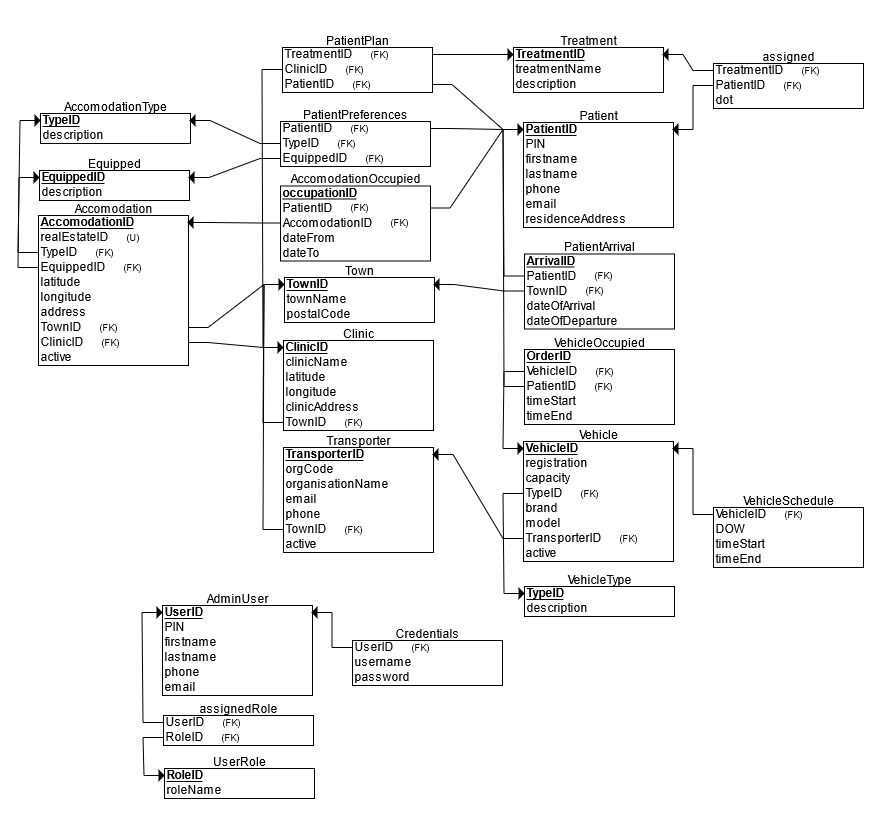
\includegraphics[width=\textwidth]{slike/DB_shema.PNG} %veličina u odnosu na širinu linije
					\caption{Sheme baze podataka}
					\label{fig:db_scheme} %label mora biti drugaciji za svaku sliku
				\end{figure}
			%Beskorisni komentar ....... :) MUAHHAHAHAH
			\eject
			
			
		\section{Dijagram razreda}
		
			\textit{Potrebno je priložiti dijagram razreda s pripadajućim opisom. Zbog preglednosti je moguće dijagram razlomiti na više njih, ali moraju biti grupirani prema sličnim razinama apstrakcije i srodnim funkcionalnostima.}\\
			
			\textbf{\textit{dio 1. revizije}}\\
			
			\textit{Prilikom prve predaje projekta, potrebno je priložiti potpuno razrađen dijagram razreda vezan uz \textbf{generičku funkcionalnost} sustava. Ostale funkcionalnosti trebaju biti idejno razrađene u dijagramu sa sljedećim komponentama: nazivi razreda, nazivi metoda i vrste pristupa metodama (npr. javni, zaštićeni), nazivi atributa razreda, veze i odnosi između razreda.}\\
			
			\textbf{\textit{dio 2. revizije}}\\			
			
			\textit{Prilikom druge predaje projekta dijagram razreda i opisi moraju odgovarati stvarnom stanju implementacije}
			
			
			
			\eject
		
		\section{Dijagram stanja}
			
			
			\textbf{\textit{dio 2. revizije}}\\
			
			\textit{Potrebno je priložiti dijagram stanja i opisati ga. Dovoljan je jedan dijagram stanja koji prikazuje \textbf{značajan dio funkcionalnosti} sustava. Na primjer, stanja korisničkog sučelja i tijek korištenja neke ključne funkcionalnosti jesu značajan dio sustava, a registracija i prijava nisu. }
			
			
			\eject 
		
		\section{Dijagram aktivnosti}
			
			\textbf{\textit{dio 2. revizije}}\\
			
			 \textit{Potrebno je priložiti dijagram aktivnosti s pripadajućim opisom. Dijagram aktivnosti treba prikazivati značajan dio sustava.}
			
			\eject
		\section{Dijagram komponenti}
		
			\textbf{\textit{dio 2. revizije}}\\
		
			 \textit{Potrebno je priložiti dijagram komponenti s pripadajućim opisom. Dijagram komponenti treba prikazivati strukturu cijele aplikacije.}